\chapter{Realisierung}
\label{chap:umsetzung}

\section{C-API}
\label{sec:capi_rel}

In folgendem Kapitel wird beschrieben wie die C-API genutzt werden konnte, um dem Roboter bestimmte Wegpunkte abzufahren.

\subsection{Beispielanwendung}
\label{sub:capi-problems_rel}

Es konnte eine Anwendung erstellt werden, dass den Roboter Initialisiert und dann in einer Schleife die Positions, Geschwindigkeits und Beschleunigungsdaten sendet. Es konnte ein Bewegungsprofil errechnet werden, dem der Roboter gefolgt ist. 
\\
Bevor man Daten vom Roboter Abfragen kann, muss eine Verbindung zum Roboter hergestellt werden, diesem einen hochfahren und initialisieren lassen. Folgend werden diese Vorgänge beschrieben.\\
Mit dem Befehl ``robotinterface\_open()'' kann die Verbindung zum Roboter hergestellt werden.
\\
Um sicher zu gehen das die Verbindung offen ist, wird in einer Schleife eine bestimmte Zeit, immer wieder abgefragt ob der Roboter verbunden ist. Falls dies nicht funktioniert, wird der Vorgang abgebrochen und das Program sollte beendet werden. Es kommt vor, dass der Roboter beim starten noch in einem Sicherheitsmodus ist. Wenn dies der Fall ist, muss der Modus abgestellt werden. Dies geht mit der Funktion ``robotinterface\_unlock\_security\_stop();''.
\\
Auch hier wird zur Sicherheit eine bestimmte Zeitschleife der Befehl wiederholt an den Roboter gesandt. Wenn der Roboter dennoch in dem Sicherheitsmodus ist, ist es möglich, dass der Notausschalter am Touch Panel aktiviert ist.
Nachdem die Verbindung offen ist, muss der Roboter mit Strom versorgt werden. Mit dem Befehl ``robotinterface\_power\_on\_robot()'' kann das bewerkstelligt werden. Auch hier wird eine bestimmte Zeitschleife abgewartet, bis der Roboter hochgefahren ist. Abgefragt werden kann dies mit der Funktion ``robotinterface\_is\_power\_on\_robot()''.

Nun wird der Roboter Initialisiert. Der Roboter geht nach dem Starten automatisch in den initialize Modus. Jeder einzelne Joint muss nun solang in eine Richtung bewegt werden, bis der Joint in den normalen Modus übergeht. Um die Gelenke zu bewegen, wird eine Geschwindigkeitsvorgabe an den Roboter gesandt.(siehe Listing \ref{lst:initialize_robot_lst})

\begin{lstlisting}[language=C,caption={Initialisierung der einzelnen Gelenke}, label=lst:initialize_robot_lst,captionpos=b]
puts("Initializing robot");
/// Set zero velocity and acceleration as guard
int j;
for (j=0; j<6; ++j) {
  pva_packet.velocity[j] = 0.0;
  pva_packet.acceleration[j] = 0.0;
}
do {
  ++i;
  robotinterface_read_state_blocking();
  int j;
  for (j=0; j<6; ++j) {
    // initialize_direction is 1 or -1. it determines in which direction die Joint is moving during the initialization
    pva_packet.velocity[j] = ((robotinterface_get_joint_mode(j) == JOINT_INITIALISATION_MODE)) ? (initialize_direction)* 0.1 : 0.0;
   }
  robotinterface_command_velocity(pva_packet.velocity);
  robotinterface_send();
} while (robotinterface_get_robot_mode() == ROBOT_INITIALIZING_MODE && exit_flag == false);
puts(" Done!");
\end{lstlisting}

Nachdem die Initialisierung abgeschlossen ist, muss wie in Listing \ref{lst:robot_control_loop} eine Schleife mit der vorgegebenen Struktur durchlaufen werden, bis das Programm beendet, oder die Verbindung zum Roboter geschlossen werden soll. Wenn dies nicht so gemacht wird, geht der Roboter automatisch in den Sicherheitsstop, da nicht innerhalb von 8 Millisekunden Nachrichten an den Roboter gesendet wurden.

Innerhalb der beiden Befehlen ``robotinterface\_read\_state\_blocking()'' und ``robotinterface\_send()'' kann nun eine Interpolation berechnet werden und die Vorgaben für Position, Geschwindigkeit und Beschleunigung an den Roboter gesandt werden(siehe Listing \ref{lst:interpolate}).

\begin{lstlisting}[language=C,caption={Interpolation eines Berechneten Weges}, label=lst:interpolate,captionpos=b]
// loop through interpolation length  
for(i=0; i < move_pva_packet.interpolations+1; i++){
  robotinterface_read_state_blocking();

  // abort interpolation if Robot is in securitystop mode
  if(robotinterface_is_security_stopped()) {
      robotinterface_get_actual_current(currents_actual);
      robotinterface_command_empty_command();
      robotinterface_send();
      break;
  }

  // get current time of interpolation 
  move_pva_packet.point_in_time= (double) i * T_IPO;

  // interpolate with sinoide profile and write result in variable move_pva_packet
  interpolation_sin_ptp(&move_pva_packet);

  // write the triple to robot
  robotinterface_command_position_velocity_acceleration(move_pva_packet.pva.position,
                                                        move_pva_packet.pva.velocity,
                                                        move_pva_packet.pva.acceleration);
  // send command to robot
  robotinterface_send();
}
\end{lstlisting}

\subsection{Aufgetretene Probleme}
\label{sub:capi-problems_rel}

Der Roboter geht ab einem bestimmten Winkel in den Sicherheitsstop. Die Abweichung der Stromstärke wird zu groß. Dies kann Analysiert werden, wenn man sich den Durchschnitt der Soll und Ist Werte der Stromstärke ansieht.(liehe Abbildung \ref{average_of_target_and_actual})

\begin{figure}[ht]
  \centering
    \includegraphics[width=0.5\textwidth]{pic/average_of_target_and_actual.png}
      \caption[Soll und Ist Werte der Stromstärke]{Abbildung zeigt die Soll und Ist Werte der Stromstärke, bis zum Sicherheitsstop des Roboters}
      \label{fig:average_of_target_and_actual}
\end{figure}

Die Abweichung ist besonders beim 2. Gelenk hoch, da dieser am meisten Gewicht tragen muss und dort die Erdanziehung am meisten wirkt. Deswegen wird angenommen, dass der Regeler die Dynamik der Gravitation nicht mitrechnet, oder falsch berechnet. Dies kann man auch beobachten, wenn man dem Roboter in einer Schleife immer die aktuellen Ist Werte mit übergibt. Der Roboter kann nicht die Aktuelle Position halten.

\section{Polyscope}
\label{sec:Polyscope_rel}

\subsection{Programmierung}
\label{programmierung_polyscope_rel}

Die Programmierung findet meist nur auf dem Touch Tablet statt. Ein neues Programm fängt mit einem leeren Ereigniss Baum an. Es kann per touch eingabe alle möglichen Funktionen, die die Script Sprache bietet dem Baum Hinzugefügt werden. Wenn das Programm abläuft, werden von der Wurzel an die Befehle abgearbeitet.
Wie in Abbildung \ref{programm_in_polyscope} zu sehen ist, ist die Ansicht des Programmbaumes sehr unübersichtlich.

\begin{figure}[ht]
  \centering
    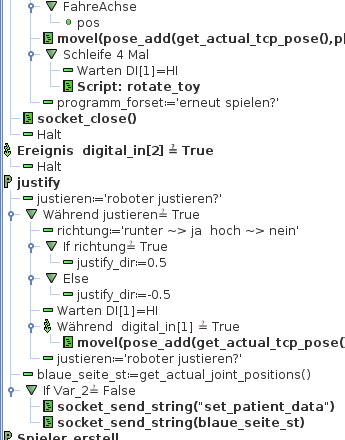
\includegraphics[width=0.5\textwidth]{pic/polyscope_program_tree.png}
      \caption[Programm Baum in Polyscope]{Ein Ausschnitt aus einem Programm Baum in Polyscope}
      \label{fig:programm_in_polyscope}
\end{figure}

Es ist möglich andere Script Dateien in das Programm einzufügen. Dazu gibt es ein feld ``Script''. Das Script Programm muss sich auf dem Linux Rechner befinden. Es ist also nötig das Script Programm auf einem anderen Rechner zu programmieren und bei jeder änderung auf den Linux Rechner des Roboters zu senden.
\\
Alternativ zu dem Touch Tablet, könnte der Xserver von dem Linux Rechner auf ein anderen Rechner umzuleiten um dort mit dem Program per Maus und Tastatur zu arbeiten. Dies wurde aber noch nicht getestet.
\\
Eine andere möglichkeit ein Programm unter Polyscope zu programmieren gibt es nicht.

\subsection{Benutzer Interaktion}
\label{user_interaktion_polyscope_rel}

Die möglichkeiten zur Interaktion mit dem Benutzer sind sehr begrenzt. Die Software und die URScript Sprache lassen es zu, dass auf dem Touch Tablet Popup Nachrichten auftauchen. Wenn man mit dem Benutzer Interagieren will, gibt mehrere Arten dieser Popups.
Als Nachricht, ja/nein Fragen, oder Text abfragen. Der Benutzer kann dann mit einen Text oder wählen zweier ja/nein buttons anworten. In Abbildung \ref{polyscope_popup} 
ist als Beispiel eine Nachricht und eine Ja/Nein Popup zu sehen.

\begin{figure}[ht]
  \centering
    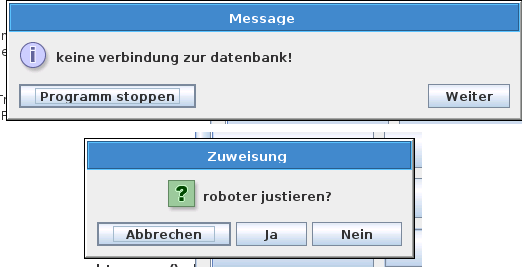
\includegraphics[width=0.8\textwidth]{pic/popup_question.png}
      \caption[Popup in Polyscipe]{Abbildung zeigt Zwei verschiedene Arten von Popups in Polyscope}
      \label{fig:polyscope_popup}
\end{figure}

Kompliziertere Menüs sind mit dieser Methode nicht möglich. Wenn ein Programm erstellt werden soll, bei dem der Benutzer viele eingaben machen muss, ist es mit Polyscope sehr schwer das zu realisieren.

\subsection{Test und Fehlersuche im Programm}
\label{debuggin_polyscope_rel}

Bevor Polyscope ein Programm ablaufen lässt wird das Script auf die richtige Syntax geprüft. Sollte ein Fehler vorhanden sein wird dies beim Start als Popup angezeigt. Fehler die in Abschnitten mit Touch hinzugefügt wurden, können jedoch nicht lokalisiert werden. Nur in extra eingefügtem Script Code kann grob lokalisiert werden, was für ein Fehler aufgetreten ist, weil dieser Teil extra geprüft wird.
\\\\
Da das Programm mit dem Touch Panel ausgeführt werden kann, ist es möglich wärend der Programmierung das Programm ablaufen zu lassen. Es kann sehr schnell getestet werden ob die gewünchten Einstellungen dem Ergebniss entsprechen. Bei Großen Programen mit vielen Benutzeranfragen, kann dies jedoch viel Zeit in anspruch nehmen. Es muss von einem Benutzer bei Jeder Anfrage eines Popups von Hand geantwortet werden.

\subsection{Aufwand der Programmierung}
\label{polyscope_aufwand}

Kleine Programme in Polyscope sind sehr schnell geschrieben. Mit dem Touch Panel kann sehr schnell eine kleine Kontrollstruktur aufgebaut werden. Das Tablet hat jedoch große Nachteile. Wie in abbildung \ref{polyscope_program_tree} zu sehen ist der Bereich für den Programm Baum sehr klein. Wenn ein Programm nun 1000 Befehle enthällt, ist es nicht möglich ein Überblick zu halten. Auch ist es sehr aufwändig zu bestimmten Bereichen hinzuspringen, da das Touch Tablet nicht genau ist. Möglich ist es geschriebene Bereiche auf Scriptdateien zu verschieben, die dann im Polyscope Programm verwendet werden. 

\subsection{TCP Server mit Datenbank zum dauerhaften speichern der Daten}
\label{tcp_datentank_sicherung_rel}

Um mit Polyscope und URScript erhobene Daten zu Speichern wurde ein kleiner TCP Server geschrieben, der eine verbindung zulässt und Daten in einer Datenbank Speichert. Die Daten sind Objectorientiert, und werden von dem Server erstellt. 
In Polyscope und URScript gibt es keine Objectorientierung, deshalb musss dort alles nacheinander angefragt werden. 


\section{URScript}
\label{sec:ur_script_rel}

Die URScriptsprache ist sehr stark an Python gelent. Es wird auf Einrückung des Textes geachtet.
Das Manual von Univeral Robots umfasst alle nötigen Funktionen um Komplexe Aufgaben zu Erfüllen.

\subsection{Laden des Scripts auf den Controller}
\label{load_script_rel}

Das Script kann nicht direkt auf dem Rechner über die Polyscope Software ausgeführt werden. Um ein selbst geschriebenes Programm in URScript auszuführen ist es nötig sich mit dem Sec
ondary Interface des URControllers \ref{urcontrol_spi_gru} per TCP zu verbinden und dann die Einzelnen Zeilen der Script Datei an den Controller zu senden.
\\\\
Es ist möglich einzelne Befehle oder ein großes Program auszuführen. Um einzelne Befehle auszuführen, werden diese nacheinander versendet.
Ein ganzes Programm wird versendet, indem wie in Listing \ref{urscipt_program_lst} gezeigt eine Funktion die ganzen Befehle umschließt. Der Controller führt diese Funktion aus, sobald diese mit dem ``end'' abgeschlossen ist.

\begin{lstlisting}[caption={Kleines Beispielprogram in URScript}, label=lst:urscipt_program_lst ,captionpos=b] 
def myProg():
	popup("hello world","test", False, False)
	set_digital_out(1, True)
	movej([0.23,1.23,0.343,0.34.0.0,0.0],a=0.5,v=0.3)
end
\end{lstlisting}

\subsection{Programmierung}
\label{programmierung_ur_script_rel}

Programmiert werden kann das Script mit allen vorhandenen Textverarbeitungsprogrammen. Vorteilhaft ist es, wenn das Programm \ac{Syntax Highlighting} für Python beherscht. Da URScript sehr stark an Python angelehnt ist, hilft dies ein wenig den Überblick zu behalten.

\subsection{Test und Fehlersuche im Programm}
\label{ur_script_debuggen}

Nach dem senden des Programms an den URController ist die einzigste möglichkeit zu sehen ob das Programm fehler enthällt, wenn der Controller kein ``Programm läuft'' Bit setzt. Man erhällt keine Nachrichten was nicht in Ordnung ist, falls das Scriptprogramm nicht abläuft.

\subsection{Benutzer Interaktion}
\label{ur_script_user_interaction}
Lorem ipsum dolor sit amet, consetetur sadipscing elitr, sed diam nonumy eirmod tempor invidunt ut labore et dolore magna aliquyam erat, sed diam voluptua. At vero eos et accusam et justo duo dolores et ea rebum. Stet clita kasd gubergren, no sea takimata sanctus est Lorem ipsum dolor sit amet. Lorem ipsum dolor sit amet, consetetur sadipscing elitr, sed diam nonumy eirmod tempor invidunt ut labore et dolore magna aliquyam erat, sed diam voluptua. At vero eos et accusam et justo duo dolores et ea rebum. Stet clita kasd gubergren, no sea takimata sanctus est Lorem ipsum dolor sit amet.

\subsection{Aufwand der Programmierung}
\label{ur_script_aufwand}

\section{Anwendung mit eigener API}
\label{sec:script_hoerherer_schicht_rel}
Lorem ipsum dolor sit amet, consetetur sadipscing elitr, sed diam nonumy eirmod tempor invidunt ut labore et dolore magna aliquyam erat, sed diam voluptua. At vero eos et accusam et justo duo dolores et ea rebum. Stet clita kasd gubergren, no sea takimata sanctus est Lorem ipsum dolor sit amet. Lorem ipsum dolor sit amet, consetetur sadipscing elitr, sed diam nonumy eirmod tempor invidunt ut labore et dolore magna aliquyam erat, sed diam voluptua. At vero eos et accusam et justo duo dolores et ea rebum. Stet clita kasd gubergren, no sea takimata sanctus est Lorem ipsum dolor sit amet.

\subsection{Adapter zur Secondary Schnittstelle}
\label{beschreibung_script_hoeher_schicht}
Lorem ipsum dolor sit amet, consetetur sadipscing elitr, sed diam nonumy eirmod tempor invidunt ut labore et dolore magna aliquyam erat, sed diam voluptua. At vero eos et accusam et justo duo dolores et ea rebum. Stet clita kasd gubergren, no sea takimata sanctus est Lorem ipsum dolor sit amet. Lorem ipsum dolor sit amet, consetetur sadipscing elitr, sed diam nonumy eirmod tempor invidunt ut labore et dolore magna aliquyam erat, sed diam voluptua. At vero eos et accusam et justo duo dolores et ea rebum. Stet clita kasd gubergren, no sea takimata sanctus est Lorem ipsum dolor sit amet.

\subsection{Programmierung mit Adapter}
\label{programmierung_mit_hoerherer_schicht}
Lorem ipsum dolor sit amet, consetetur sadipscing elitr, sed diam nonumy eirmod tempor invidunt ut labore et dolore magna aliquyam erat, sed diam voluptua. At vero eos et accusam et justo duo dolores et ea rebum. Stet clita kasd gubergren, no sea takimata sanctus est Lorem ipsum dolor sit amet. Lorem ipsum dolor sit amet, consetetur sadipscing elitr, sed diam nonumy eirmod tempor invidunt ut labore et dolore magna aliquyam erat, sed diam voluptua. At vero eos et accusam et justo duo dolores et ea rebum. Stet clita kasd gubergren, no sea takimata sanctus est Lorem ipsum dolor sit amet.

\subsection{Benutzer Interaktion}
\label{user_interaktion_mit_hoerherer_schicht}

Lorem ipsum dolor sit amet, consetetur sadipscing elitr, sed diam nonumy eirmod tempor invidunt ut labore et dolore magna aliquyam erat, sed diam voluptua. At vero eos et accusam et justo duo dolores et ea rebum. Stet clita kasd gubergren, no sea takimata sanctus est Lorem ipsum dolor sit amet. Lorem ipsum dolor sit amet, consetetur sadipscing elitr, sed diam nonumy eirmod tempor invidunt ut labore et dolore magna aliquyam erat, sed diam voluptua. At vero eos et accusam et justo duo dolores et ea rebum. Stet clita kasd gubergren, no sea takimata sanctus est Lorem ipsum dolor sit amet.

\subsection{Test und Fehlersuche im Programm}
\label{debuggen_mit_hoeherer schicht}
Lorem ipsum dolor sit amet, consetetur sadipscing elitr, sed diam nonumy eirmod tempor invidunt ut labore et dolore magna aliquyam erat, sed diam voluptua. At vero eos et accusam et justo duo dolores et ea rebum. Stet clita kasd gubergren, no sea takimata sanctus est Lorem ipsum dolor sit amet. Lorem ipsum dolor sit amet, consetetur sadipscing elitr, sed diam nonumy eirmod tempor invidunt ut labore et dolore magna aliquyam erat, sed diam voluptua. At vero eos et accusam et justo duo dolores et ea rebum. Stet clita kasd gubergren, no sea takimata sanctus est Lorem ipsum dolor sit amet.

\subsection{Aufwand der Programmierung}
\label{eigene_api_aufwand}